\documentclass[twocolumn]{article}
\usepackage[utf8]{inputenc}
\usepackage[top=1in]{geometry}
\usepackage{graphicx}
\usepackage{hyperref}
\usepackage{amsmath}
% Calligraphic fonts
\newcommand{\calA}{{\cal A}}
\newcommand{\calB}{{\cal B}}
\newcommand{\calC}{{\cal C}}
\newcommand{\calD}{{\cal D}}
\newcommand{\calE}{{\cal E}}
\newcommand{\calF}{{\cal F}}
\newcommand{\calG}{{\cal G}}
\newcommand{\calH}{{\cal H}}
\newcommand{\calI}{{\cal I}}
\newcommand{\calJ}{{\cal J}}
\newcommand{\calK}{{\cal K}}
\newcommand{\calL}{{\cal L}}
\newcommand{\calM}{{\cal M}}
\newcommand{\calN}{{\cal N}}
\newcommand{\calO}{{\cal O}}
\newcommand{\calP}{{\cal P}}
\newcommand{\calQ}{{\cal Q}}
\newcommand{\calR}{{\cal R}}
\newcommand{\calS}{{\cal S}}
\newcommand{\calT}{{\cal T}}
\newcommand{\calU}{{\cal U}}
\newcommand{\calV}{{\cal V}}
\newcommand{\calW}{{\cal W}}
\newcommand{\calX}{{\cal X}}
\newcommand{\calY}{{\cal Y}}
\newcommand{\calZ}{{\cal Z}}

% Sets:
\newcommand{\setA}{\textsf{A}}
\newcommand{\setB}{\textsf{B}}
\newcommand{\setC}{\textsf{C}}
\newcommand{\setD}{\textsf{D}}
\newcommand{\setE}{\textsf{E}}
\newcommand{\setF}{\textsf{F}}
\newcommand{\setG}{\textsf{G}}
\newcommand{\setH}{\textsf{H}}
\newcommand{\setI}{\textsf{I}}
\newcommand{\setJ}{\textsf{J}}
\newcommand{\setK}{\textsf{K}}
\newcommand{\setL}{\textsf{L}}
\newcommand{\setM}{\textsf{M}}
\newcommand{\setN}{\textsf{N}}
\newcommand{\setO}{\textsf{O}}
\newcommand{\setP}{\textsf{P}}
\newcommand{\setQ}{\textsf{Q}}
\newcommand{\setR}{\textsf{R}}
\newcommand{\setS}{\textsf{S}}
\newcommand{\setT}{\textsf{T}}
\newcommand{\setU}{\textsf{U}}
\newcommand{\setV}{\textsf{V}}
\newcommand{\setW}{\textsf{W}}
\newcommand{\setX}{\textsf{X}}
\newcommand{\setY}{\textsf{Y}}
\newcommand{\setZ}{\textsf{Z}}

% Vectors
\newcommand{\bfa}{\mathbf{a}}
\newcommand{\bfb}{\mathbf{b}}
\newcommand{\bfc}{\mathbf{c}}
\newcommand{\bfd}{\mathbf{d}}
\newcommand{\bfe}{\mathbf{e}}
\newcommand{\bff}{\mathbf{f}}
\newcommand{\bfg}{\mathbf{g}}
\newcommand{\bfh}{\mathbf{h}}
\newcommand{\bfi}{\mathbf{i}}
\newcommand{\bfj}{\mathbf{j}}
\newcommand{\bfk}{\mathbf{k}}
\newcommand{\bfl}{\mathbf{l}}
\newcommand{\bfm}{\mathbf{m}}
\newcommand{\bfn}{\mathbf{n}}
\newcommand{\bfo}{\mathbf{o}}
\newcommand{\bfp}{\mathbf{p}}
\newcommand{\bfq}{\mathbf{q}}
\newcommand{\bfr}{\mathbf{r}}
\newcommand{\bfs}{\mathbf{s}}
\newcommand{\bft}{\mathbf{t}}
\newcommand{\bfu}{\mathbf{u}}
\newcommand{\bfv}{\mathbf{v}}
\newcommand{\bfw}{\mathbf{w}}
\newcommand{\bfx}{\mathbf{x}}
\newcommand{\bfy}{\mathbf{y}}
\newcommand{\bfz}{\mathbf{z}}


\newcommand{\bfalpha}{\boldsymbol{\alpha}}
\newcommand{\bfbeta}{\boldsymbol{\beta}}
\newcommand{\bfgamma}{\boldsymbol{\gamma}}
\newcommand{\bfdelta}{\boldsymbol{\delta}}
\newcommand{\bfepsilon}{\boldsymbol{\epsilon}}
\newcommand{\bfzeta}{\boldsymbol{\zeta}}
\newcommand{\bfeta}{\boldsymbol{\eta}}
\newcommand{\bftheta}{\boldsymbol{\theta}}
\newcommand{\bfiota}{\boldsymbol{\iota}}
\newcommand{\bfkappa}{\boldsymbol{\kappa}}
\newcommand{\bflambda}{\boldsymbol{\lambda}}
\newcommand{\bfmu}{\boldsymbol{\mu}}
\newcommand{\bfnu}{\boldsymbol{\nu}}
\newcommand{\bfomicron}{\boldsymbol{\omicron}}
\newcommand{\bfpi}{\boldsymbol{\pi}}
\newcommand{\bfrho}{\boldsymbol{\rho}}
\newcommand{\bfsigma}{\boldsymbol{\sigma}}
\newcommand{\bftau}{\boldsymbol{\tau}}
\newcommand{\bfupsilon}{\boldsymbol{\upsilon}}
\newcommand{\bfphi}{\boldsymbol{\phi}}
\newcommand{\bfchi}{\boldsymbol{\chi}}
\newcommand{\bfpsi}{\boldsymbol{\psi}}
\newcommand{\bfomega}{\boldsymbol{\omega}}
\newcommand{\bfxi}{\boldsymbol{\xi}}
\newcommand{\bfell}{\boldsymbol{\ell}}

% Matrices
\newcommand{\bfA}{\mathbf{A}}
\newcommand{\bfB}{\mathbf{B}}
\newcommand{\bfC}{\mathbf{C}}
\newcommand{\bfD}{\mathbf{D}}
\newcommand{\bfE}{\mathbf{E}}
\newcommand{\bfF}{\mathbf{F}}
\newcommand{\bfG}{\mathbf{G}}
\newcommand{\bfH}{\mathbf{H}}
\newcommand{\bfI}{\mathbf{I}}
\newcommand{\bfJ}{\mathbf{J}}
\newcommand{\bfK}{\mathbf{K}}
\newcommand{\bfL}{\mathbf{L}}
\newcommand{\bfM}{\mathbf{M}}
\newcommand{\bfN}{\mathbf{N}}
\newcommand{\bfO}{\mathbf{O}}
\newcommand{\bfP}{\mathbf{P}}
\newcommand{\bfQ}{\mathbf{Q}}
\newcommand{\bfR}{\mathbf{R}}
\newcommand{\bfS}{\mathbf{S}}
\newcommand{\bfT}{\mathbf{T}}
\newcommand{\bfU}{\mathbf{U}}
\newcommand{\bfV}{\mathbf{V}}
\newcommand{\bfW}{\mathbf{W}}
\newcommand{\bfX}{\mathbf{X}}
\newcommand{\bfY}{\mathbf{Y}}
\newcommand{\bfZ}{\mathbf{Z}}


\newcommand{\bfGamma}{\boldsymbol{\Gamma}}
\newcommand{\bfDelta}{\boldsymbol{\Delta}}
\newcommand{\bfTheta}{\boldsymbol{\Theta}}
\newcommand{\bfLambda}{\boldsymbol{\Lambda}}
\newcommand{\bfPi}{\boldsymbol{\Pi}}
\newcommand{\bfSigma}{\boldsymbol{\Sigma}}
\newcommand{\bfUpsilon}{\boldsymbol{\Upsilon}}
\newcommand{\bfPhi}{\boldsymbol{\Phi}}
\newcommand{\bfPsi}{\boldsymbol{\Psi}}
\newcommand{\bfOmega}{\boldsymbol{\Omega}}


% Blackboard Bold:
\newcommand{\bbA}{\mathbb{A}}
\newcommand{\bbB}{\mathbb{B}}
\newcommand{\bbC}{\mathbb{C}}
\newcommand{\bbD}{\mathbb{D}}
\newcommand{\bbE}{\mathbb{E}}
\newcommand{\bbF}{\mathbb{F}}
\newcommand{\bbG}{\mathbb{G}}
\newcommand{\bbH}{\mathbb{H}}
\newcommand{\bbI}{\mathbb{I}}
\newcommand{\bbJ}{\mathbb{J}}
\newcommand{\bbK}{\mathbb{K}}
\newcommand{\bbL}{\mathbb{L}}
\newcommand{\bbM}{\mathbb{M}}
\newcommand{\bbN}{\mathbb{N}}
\newcommand{\bbO}{\mathbb{O}}
\newcommand{\bbP}{\mathbb{P}}
\newcommand{\bbQ}{\mathbb{Q}}
\newcommand{\bbR}{\mathbb{R}}
\newcommand{\bbS}{\mathbb{S}}
\newcommand{\bbT}{\mathbb{T}}
\newcommand{\bbU}{\mathbb{U}}
\newcommand{\bbV}{\mathbb{V}}
\newcommand{\bbW}{\mathbb{W}}
\newcommand{\bbX}{\mathbb{X}}
\newcommand{\bbY}{\mathbb{Y}}
\newcommand{\bbZ}{\mathbb{Z}}




\title{ECE 417/598: Homework 2}
\date{Due on Feb 4th, 2021, before class, 12:59 PM.}
\newtheorem{prob}{Problem}

\newcommand{\bx}{\bar{x}}
\newcommand{\by}{\bar{y}}
\newcommand{\bz}{\bar{z}}
\begin{document}

\maketitle
\section{Jan 26 Lecture}

\begin{prob}
  In class we proved the Rodrigues formula that converts from axis-angle
  representation $(\theta, \hat{\bfk})$, where $\theta$ is the angle of rotation
  and $\hat{\bfk}$ is the axis of rotation. Let $\bfK = [\hat{\bfk}]_{\times}$ be
  the cross product matrix of $\hat{\bfk}$. The corresponding rotation matrix is
  given by,
  \begin{align}
    R(\theta, \hat{\bfk}) = \bfI + \sin \theta \bfK + (1-cos \theta) \bfK^2.
  \end{align}

  An exponential of a square matrix $\bfM$ is defined as
  \begin{align}
    \exp(\bfM) = \sum_{n=0}^\infty \frac{1}{n!} \bfM^k = \bfI + \frac{1}{1!}\bfM + \frac{1}{2!}\bfM^2 + \dots
  \end{align}

  Recall the series expansion of $\sin \theta$, and $\cos \theta$,
  \begin{align}
    \sin \theta = \theta - \frac{\theta^3}{3!} + \frac{\theta^5}{5!} - \dots
    \\
    \cos \theta = 1 - \frac{\theta^2}{2!} + \frac{\theta^4}{3!} - \dots
  \end{align}
\end{prob}

  \begin{enumerate}
   \item First prove that $\bfK^3 = - \bfK$. (10 marks, 10 minutes)
   \item Using the expansion of $\sin\theta$ and $\cos\theta$, prove that
     $R(\theta, \hat{\bfk}) = \exp(\theta \bfK)$. (30 marks, 30 minutes)
  \end{enumerate}

\begin{prob}
  Write a pair of functions in C++ that converts rotation matrix from axis-angle
  representation and vice versa. Recall that
  \begin{align}
    R(\theta, \hat{\bfk}) = \bfI + \sin \theta \bfK + (1-cos \theta) \bfK^2.
  \end{align}
  and to get axis-angle back from a given rotation matrix
  \begin{align}
    R = \begin{bmatrix}
      r_{11} & r_{12} & r_{13} \\
      r_{21} & r_{22} & r_{23} \\
      r_{31} & r_{32} & r_{33}
      \end{bmatrix},
  \end{align}
  we have
  \begin{align}
    \theta &= \cos^{-1} \left(\frac{\text{tr}(R) - 1}{2}\right)
    \\
    \hat{\bfk} &= \frac{1}{2\sin\theta}\begin{bmatrix}
      r_{32} - r_{23} \\
      r_{13} - r_{31} \\
      r_{21} - r_{12}
      \end{bmatrix} \text{ if  } \theta \ne 0 \text{ or } \pi.
  \end{align}
 If $\theta = 0 \text{ or } \pi$, then
 \begin{align}
   \hat{\bfk} = \pm\begin{bmatrix}
    \sqrt{(r_{11} + 1)/2}\\
    \sqrt{(r_{22} + 1)/2}\\
    \sqrt{(r_{33} + 1)/2}
   \end{bmatrix}
   \end{align}
  
  (30 marks. Estimated time: 30 min)
  \label{prob:euler-to-rotmat}
\end{prob}


\section{Jan 31 Lecture}
\begin{prob}
  Recall the definition of Denavit-Hartenberg parameters from the
  \href{https://www.youtube.com/watch?v=rA9tm0gTln8}{video}. Recall that
  transformation between two joints for the defined parameters $d, \theta, r,
  \alpha$ is given by,
  \begin{align}
    T = T_z(\theta, d) T_x(\alpha, r),
  \end{align}
  where
  \begin{align}
    T_x(\alpha, r) &= \begin{bmatrix}
      1 & 0 & 0 & r \\
      0 & \cos(\alpha) & -\sin(\alpha) & 0 \\
      0 & \sin(\alpha) & \cos(\alpha) & 0 \\
      0 & 0 & 0 & 1 \\
      \end{bmatrix}
    \\
    T_z(\theta, d) &= \begin{bmatrix}
      \cos(\theta) & -\sin(\theta) & 0 &  0 \\
      \sin(\theta) & \cos(\theta) & 0  & 0 \\
      0 & 0 & 1 & d & \\
      0 & 0 & 0 & 1 &
    \end{bmatrix}
  \end{align}

  For the robot given below find transformation matrix from joint 4 to joint 1
  assuming the joint angles to be  $\theta_1$, $\theta_2$, $\theta_3$
  respectively. Write the expression for ${}^3T_4(\theta_3)$, ${}^2T_3(\theta_2)$, ${}^1T_2(\theta_1)$
  and then ${}^1T_4(\theta_1, \theta_2, \theta_3)$ in terms of the first three transformations.
  \\
  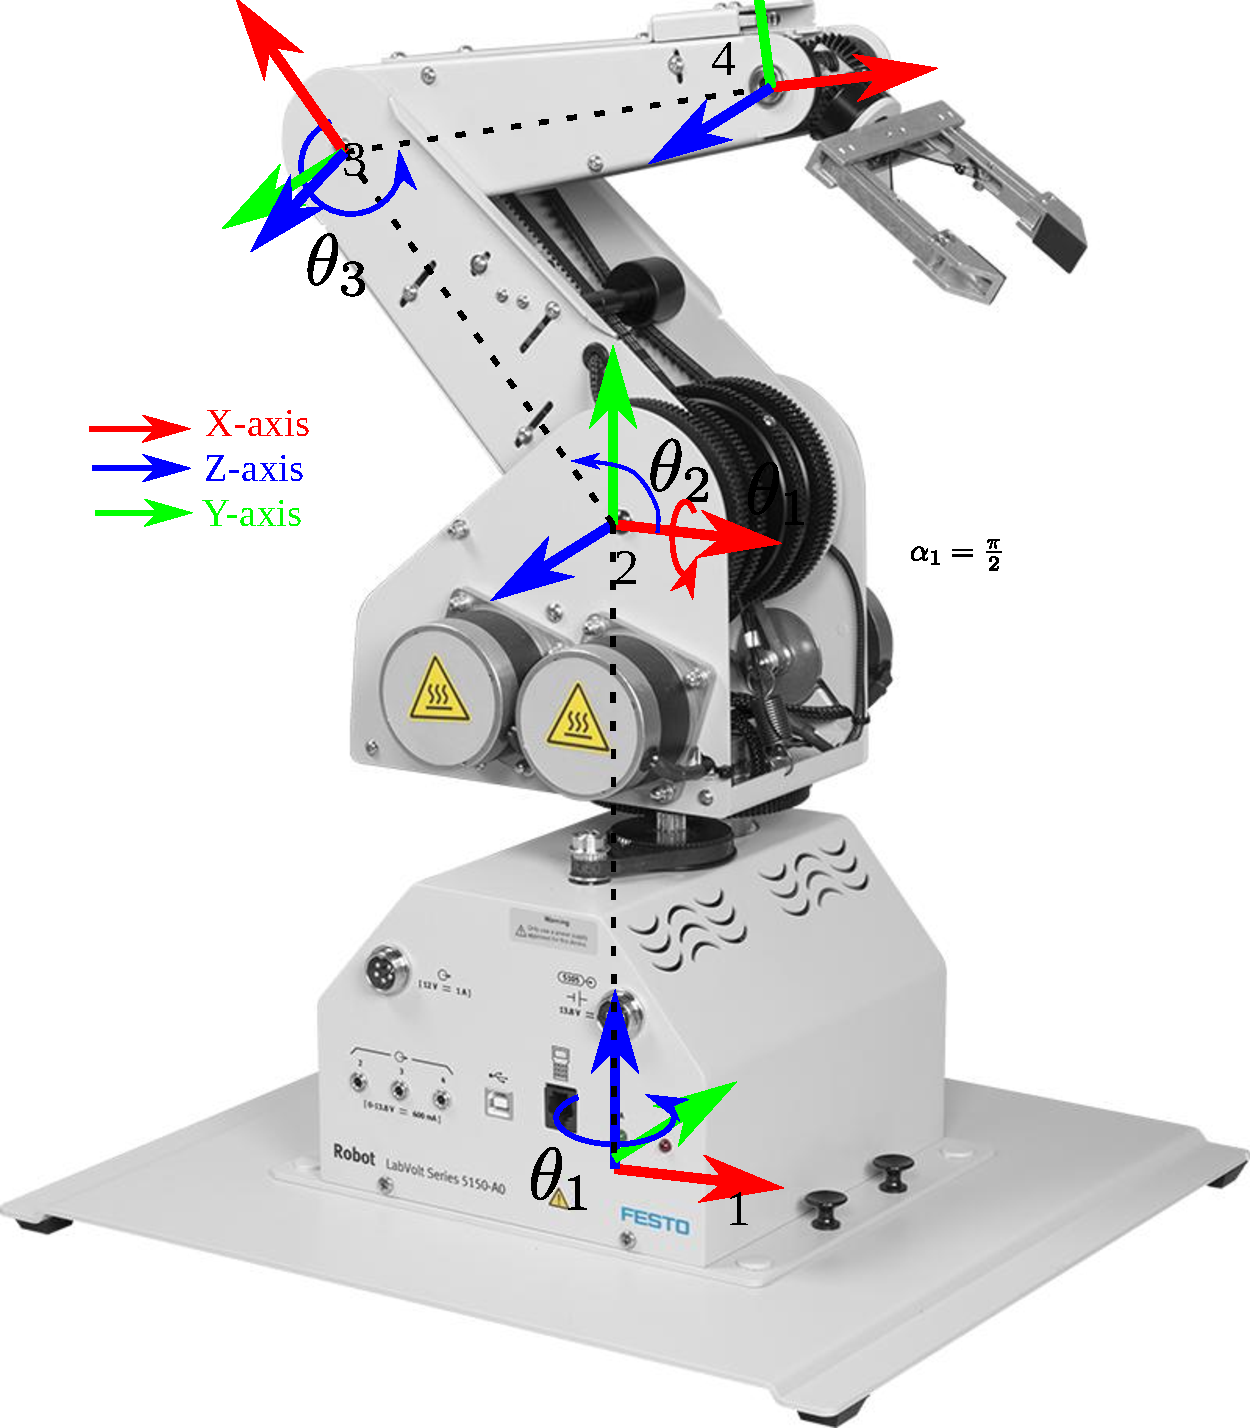
\includegraphics[width=\linewidth]{robot3D.pdf}
  \\
  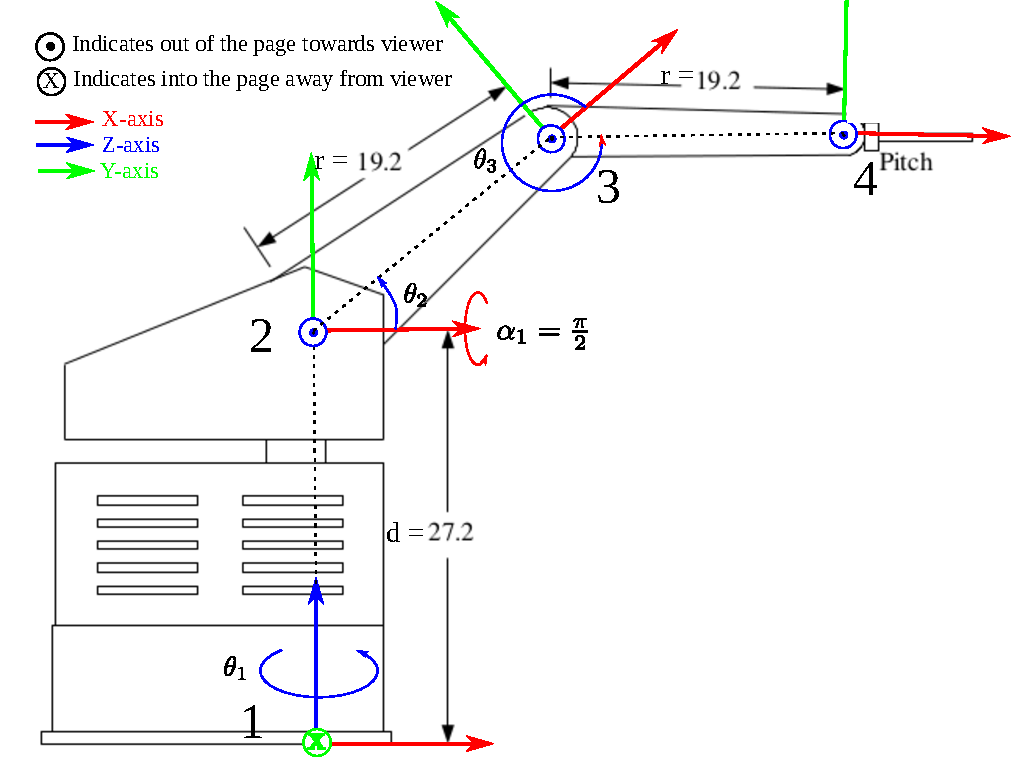
\includegraphics[width=\linewidth]{robot.pdf}
\end{prob}

\section{ECE 598 only}

Write a short review of the following paper
\href{https://openaccess.thecvf.com/content_CVPR_2019/html/Zhou_On_the_Continuity_of_Rotation_Representations_in_Neural_Networks_CVPR_2019_paper.html}{On
  continuity of rotation representations in Neural networks}. We have not
covered all the concepts covered in this paper; you can skip the parts that you
do not understand. In the review answer the following questions evaluating the paper,
\begin{enumerate}
\item Problem: What problem is the paper trying to solve?
\item Approach: What is the proposed approach to solve the problem?
\item Contribution: What is the paper's novel contribution?
\item Evidence: Do they any experiments or proof that their approach/contributions work?
\item Results: Are the results of the paper justified by evidence and a direct
  result of the contibutions?
\end{enumerate}

%\bibliography{main}
%\bibliographystyle{plain}
\end{document}